\documentclass[11pt]{article}
\usepackage[margin=1in]{geometry}
\usepackage[T1]{fontenc}
\usepackage{lmodern}
\usepackage{amsmath}
\usepackage{graphicx}
\usepackage{caption}
\usepackage{booktabs}
\usepackage[hidelinks]{hyperref}
\newcommand{\tauR}{Tau-5$_{\mathrm{R2}}$}
\captionsetup{font=small,labelfont=bf}
\renewcommand{\figurename}{Supporting Figure}
\renewcommand{\thefigure}{S\arabic{figure}}
\renewcommand{\tablename}{Supporting Table}
\renewcommand{\thetable}{S\arabic{table}}
\setcounter{figure}{1}
\setcounter{table}{0}
\begin{document}

\section*{Analysis of the kinetics of \tauR{} self-association}

We characterized the kinetics of \tauR{} self-association in the apo, EPI-002, and 1aa simulations using binary time series sampled at 0.24-ns intervals. Each frame was classified as bound when at least one intermolecular C$\alpha$--C$\alpha$ minimum-image distance was less than 10~\AA{} and as unbound otherwise. We used these assignments to calculate dimer-state autocorrelation functions, distributions of consecutive bound-state durations, and waiting times for reassociation following dissociation. Supporting Figure~\ref{fig:kinetics} shows the event-duration and reassociation distributions. Consecutive bound or unbound episodes were defined at the saved-frame resolution; transitions occurring between successive saved frames were not resolved.

\subsection*{Double-exponential fitting of dimer-state autocorrelation functions}

Dimer contact persistence autocorrelation functions, $C(t)$, were computed from the binary dimer self-association time series, where frames containing intermolecular contacts between \tauR{} monomers were represented by a value of 1, and frames with no intermolecular contacts were represented by a value of 0. These functions quantify correlations in the association state at time points separated by a given lag time, allowing intervening dissociation and reassociation. The time-series mean was subtracted before calculating the autocorrelation, the covariance at each lag was averaged over all available frame pairs, and the result was divided by the variance of the binary time series so that $C(0)=1$. Each $C(t)$ was fit to a double-exponential decay:
\begin{equation}
C(t)=a_{\mathrm{fast}}\exp\left(-\frac{t}{\tau_{\mathrm{fast}}}\right)
+a_{\mathrm{slow}}\exp\left(-\frac{t}{\tau_{\mathrm{slow}}}\right).
\end{equation}
Here, $a_{\mathrm{fast}}$ and $a_{\mathrm{slow}}$ are the fitted amplitudes, and $\tau_{\mathrm{fast}}$ and $\tau_{\mathrm{slow}}$ are the corresponding correlation times. Amplitudes and correlation times were constrained to be non-negative; the amplitudes were not constrained to sum to one. Fits were obtained by unweighted nonlinear least squares over lag times from 0 to 1.99992~$\mu$s. The fitted correlation times describe association-state relaxation rather than continuous dimer lifetimes. Fit parameters are reported in Supporting Table~\ref{tab:fits}.

\subsection*{Dissociation and Association Kinetics}

Using the same binary dimer self-association time series, we identified individual dimer-binding events as consecutive frames with a value of 1. Each event ended at the first subsequent frame with a value of 0. The observed duration of each event was calculated by multiplying the number of consecutive bound frames by the 0.24-ns frame spacing. Panel A shows the number of events in each duration range. The final 1aa dimer remained associated when the trajectory ended, after 37.92744~$\mu$s of observed binding. This event is included according to its observed duration and distinguished by an asterisk above the bar; its complete lifetime is unknown.

To describe the distribution of dimer-state lifetimes, we calculated the fraction of binding events that remained associated as a function of time since association. Each curve begins at 1 and decreases when an observed binding event ends. At each event duration, the preceding survival fraction is multiplied by one minus the fraction of events still being followed that dissociate at that duration. An event that remains bound at the end of the trajectory contributes to the calculation for as long as it is observed, but its endpoint is not counted as a dissociation. Panel B shows the initial decay with a logarithmic time axis in nanoseconds, while panel C shows the same distribution on a logarithmic vertical axis to resolve the long-lived events. The asterisk on the 1aa curve marks the event that remained associated after 37.92744~$\mu$s of observation; the plateau does not establish how much longer this dimer would persist.

We calculated reassociation times from consecutive frames with a value of 0 following a dimer dissociation. Each unbound event ended at the first subsequent frame with a value of 1, and its duration was calculated by multiplying the number of consecutive unbound frames by 0.24~ns. The initial unbound segment of each trajectory was excluded because its preceding dissociation was not observed. Unbound events that continued to the trajectory endpoint were included for their observed durations, without treating the endpoint as a reassociation. Thus, these curves describe waiting times for the two \tauR{} monomers to reassociate within their simulation box.

Because the 1aa simulation used a larger box and therefore a lower protein concentration, we expressed the unbound durations at the apo simulation's partner concentration. For each frame, the concentration of the single available binding partner was calculated as $1/(N_A V)$, where $V$ is the simulation-box volume in litres and $N_A$ is Avogadro's constant. Each unbound duration was rescaled by summing the framewise partner concentrations over that event, multiplying by the 0.24-ns frame spacing, and dividing by the mean apo partner concentration. For a constant box volume, this is equivalent to multiplying the unbound duration by the ratio of the simulation's partner concentration to the apo partner concentration. Panel D shows the fraction of events remaining unbound as a function of these rescaled durations, calculated using the same procedure as the dimer-survival curves. This correction assumes that the association frequency is proportional to partner concentration; it provides a comparison at a common concentration without establishing an intrinsic bimolecular association rate constant. The mean partner concentrations were 3.327, 3.331, and 1.280~mM for apo, EPI-002, and 1aa, respectively. Consequently, the correction leaves the EPI-002 durations nearly unchanged and scales the 1aa durations by approximately 0.385.

\begin{table}[htbp]
\centering
\caption{Double-exponential fit parameters for \tauR{} dimer-state autocorrelation functions sampled at 0.24-ns intervals. Uncertainties are nominal $\pm1\sigma$ standard errors from the nonlinear least-squares covariance matrix. These quantify fit precision and do not account for correlations among lag points or finite-trajectory sampling uncertainty.}
\label{tab:fits}
\small
\begin{tabular}{lccccc}
\toprule
System & $a_{\mathrm{fast}}$ & $\tau_{\mathrm{fast}}$ (ns) & $a_{\mathrm{slow}}$ & $\tau_{\mathrm{slow}}$ ($\mu$s) & $R^2$ \\
\midrule
Apo & $0.4192 \pm 0.0017$ & $56.10 \pm 0.44$ & $0.4580 \pm 0.0011$ & $0.5922 \pm 0.0014$ & 0.9936 \\
EPI-002 & $0.5199 \pm 0.0020$ & $105.31 \pm 0.77$ & $0.3495 \pm 0.0010$ & $2.6171 \pm 0.0170$ & 0.9726 \\
1aa & $0.4847 \pm 0.0010$ & $227.09 \pm 0.99$ & $0.4954 \pm 0.0009$ & $5.1780 \pm 0.0349$ & 0.9939 \\
\bottomrule
\end{tabular}
\end{table}

\clearpage
\begin{figure}[p]
\centering
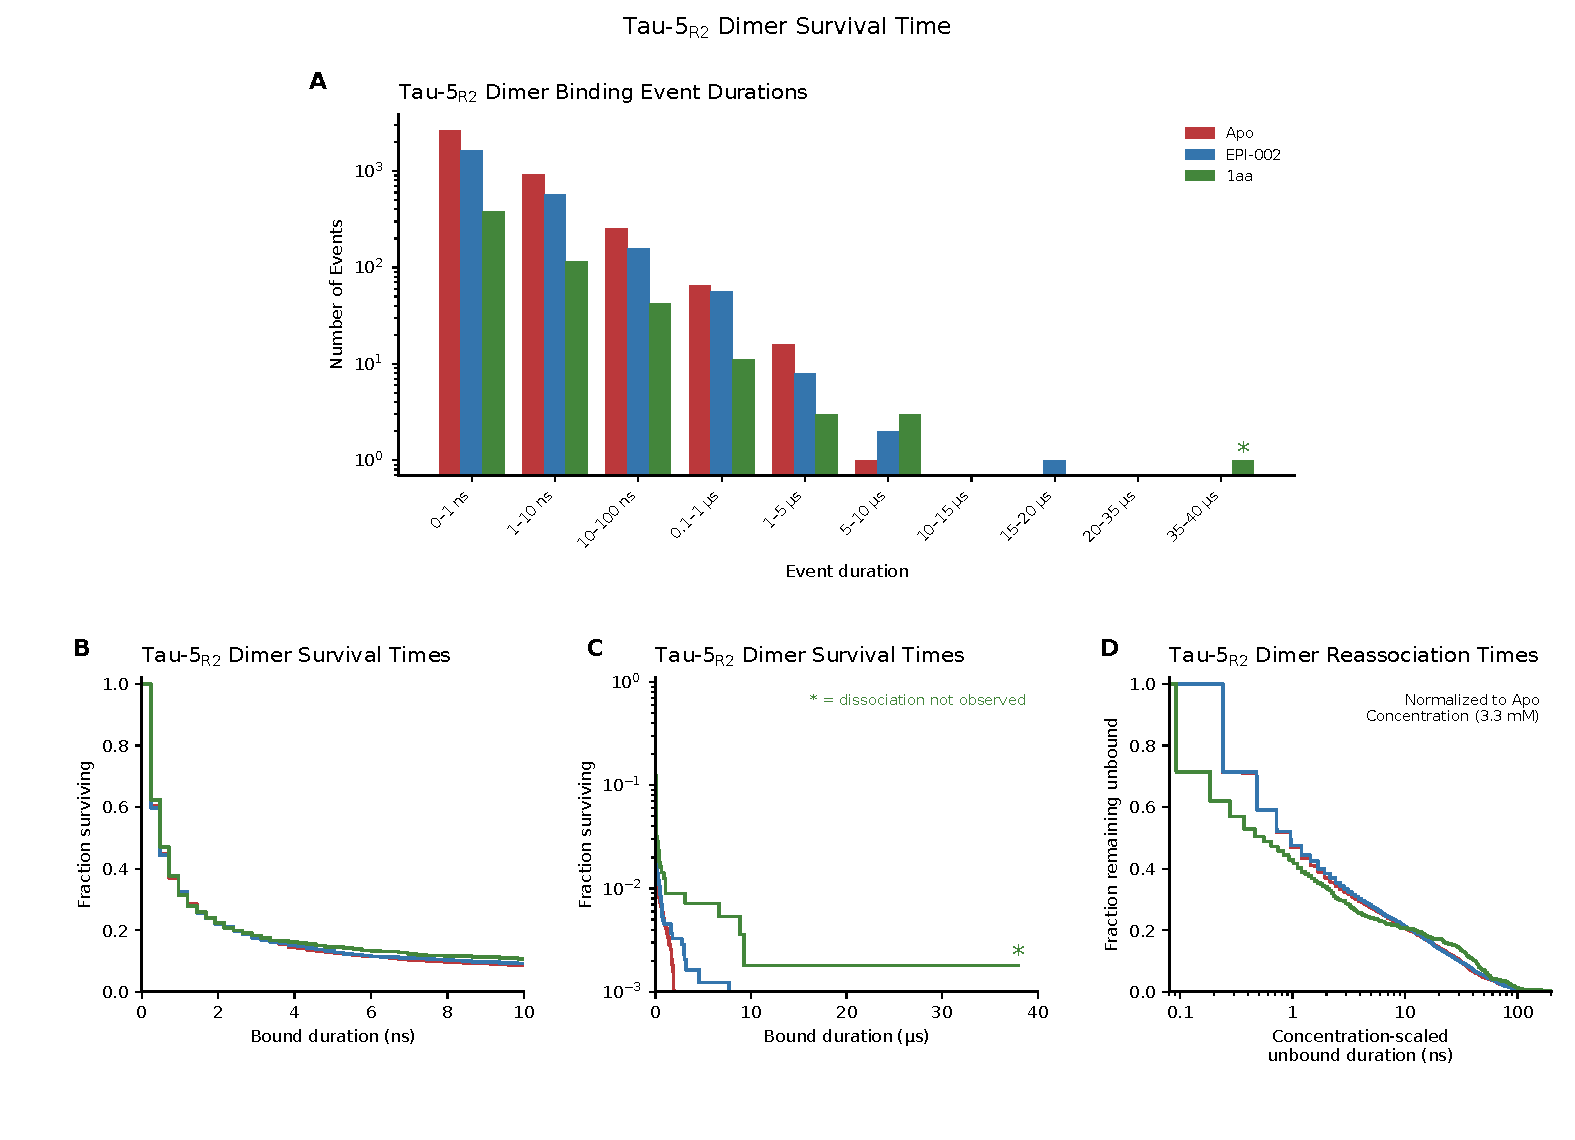
\includegraphics[width=\textwidth,height=0.53\textheight,keepaspectratio]{Figure_S2.pdf}
\caption{\textbf{\tauR{} Dimer Survival Time.} (\textbf{A}) Histogram of observed \tauR{} dimer binding-event durations in apo simulations (red) and simulations with EPI-002 (blue) or 1aa (green). The asterisk above the bar marks the final 1aa event, which remained associated for at least 37.92744~$\mu$s; dissociation was not observed. (\textbf{B}) Fraction of dimer-binding events remaining associated as a function of time since association, shown with a logarithmic time axis in nanoseconds. (\textbf{C}) The same survival curves on a logarithmic vertical axis to show the long-lived tail. The asterisk directly above the line endpoint marks the event for which dissociation was not observed. (\textbf{D}) Fraction of unbound events remaining unbound, shown with a logarithmic time axis in nanoseconds, after rescaling their durations by their integrated partner concentration relative to the mean apo partner concentration (3.3~mM). The larger simulation box used for 1aa gives a lower mean concentration of the single available binding partner (1.3~mM) than in the apo and EPI-002 simulations (both 3.3~mM). To account for this difference, each unbound duration was weighted by the partner concentration over that event and divided by the mean apo partner concentration, assuming association frequency is proportional to partner concentration. This scales the 1aa waiting times by approximately 0.385 and leaves the EPI-002 waiting times nearly unchanged. Frames were sampled every 0.24~ns. A bound frame contains at least one intermolecular C$\alpha$--C$\alpha$ minimum-image distance below 10~\AA{}. Continuous events refer to consecutive saved frames; transitions between saved frames are unresolved. Events ongoing at the trajectory endpoint contribute for their observed durations without treating the endpoint as a dissociation or reassociation. The initial unbound segment of each trajectory is excluded from reassociation distributions.}
\label{fig:kinetics}
\end{figure}
\end{document}
